\section{Observation, precision and retained computational evidence}\label{sec:observations}
\subsection{The inherited observation map}
For a fixed exterior centre $X$, orthonormal frame $B_X$, tangent $\hat t(s)$ and distance $d_X(s)=\norm{X-\Gamma(s)}$, C6 adopts
\begin{equation}\label{eq:C6}
 \begin{aligned}
 U_X(t)&=\frac{g_o}{4\pi}\int_\Gamma\frac{p(s,t-d_X(s)/c_e)}{d_X(s)}\dd s,\\
 V_X(t)&=\frac{g_o}{4\pi}\int_\Gamma\frac{r(s,t-d_X(s)/c_e)\hat t(s)}{d_X(s)}\dd s,
 \qquad Y_X=(U_X,B_X^{\mathrm T}V_X).
 \end{aligned}
\end{equation}
This assumed straight-line delay and tangent-weighted reception does not feed back into C1. The centre-sampled observer geometry and all H/R arrays are those of Paper II. No new spoke, attachment or native coupling is inferred here. In normalized output units $g_oF_0/c$, the complete late residual record has the form
\begin{equation}\label{eq:record}
 Y(\tau)=D_o\mu+\operatorname{Re}\{Q u\,e^{2\pi\ii\tau}\},\qquad u=(u_+,u_-)^{\mathrm T}.
\end{equation}
For one site the two columns of $Q$ are
\[
 Q_\sigma=\frac1{4\pi}\int_\Gamma
 \frac{e^{-\sigma\ii\chi-\ii\beta d_X}}{d_X}
 \begin{pmatrix}1\\\sigma B_X^{\mathrm T}\hat t\end{pmatrix}\dd s,
 \quad \beta=\frac{c/R}{c_e}.
\]
The negative delay phase and signed vector column have different origins. $D_o$ is the mean-field reception vector. These matrices already include retarded spatial phase; synthesis adds no second delay.

Paper II proves complex rank two for a full off-circle site when $0\le\nu=c/c_e<\pi/2$, including $\nu=0,1$. Its circular symmetry reduction gives singular values $\sqrt{2(|H_o|^2+|S_o|^2)}$ and $\sqrt2|C_o|$ in unit gain, where $H_o,S_o,C_o$ are weighted cosine, sine-squared and cosine-squared moments. Equatorial scalar rows alone coincide in the directional columns: the odd sine integrand vanishes. Every equatorial scalar array is therefore rank one, even if many radii are present. A mirror pair off the equator or a calibrated full vector/scalar site can supply the missing complex direction. These are inherited rank statements, not new array optimization.

\begin{proposition}[Common phase/gain and sampled inversion]\label{prop:observation}
Suppose a known complex matrix $Q$ has rank two and samples are taken at $\tau_0+k/n$, $k=0,\ldots,n-1$, with $n\ge3$ and the usual DC, cosine and sine columns independent. In an exact first-harmonic record, fitting those columns gives phasor
\begin{equation}\label{eq:extraction}
 \widehat Y=(a_{\cos}-\ii a_{\sin})e^{-2\pi\ii\tau_0}.
\end{equation}
If all harmonic channels share an unknown factor $\gamma\ne0$, applying $Q^\dagger$ returns $\gamma u$, and $\etaosc$ is unchanged. The moment decoder may instead invert $Q\Mat$ and use \eqref{eq:momentread}.
\end{proposition}
\begin{proof}
For complex $h$, $\operatorname{Re}(he^{2\pi\ii k/n})=(\operatorname{Re}h)\cos(2\pi k/n)-(\operatorname{Im}h)\sin(2\pi k/n)$. At the common window origin $h=Q u e^{2\pi\ii\tau_0}$, proving the extraction sign and rotation. Full column rank gives $Q^\dagger Q=I$, hence $Q^\dagger(\gamma Q u)=\gamma u$. The common $|\gamma|^2$ cancels from the ratio. Invertibility of $\Mat$ proves the analogous moment statement. Independently unknown channel gains or clocks cannot generally be factored into one $\gamma$, so the conclusion does not extend to them.
\end{proof}
The retained interface uses eight equally spaced samples over one period with endpoint omitted. A clean 16-sample control is also retained. The window begins after the latest event end plus $D_{\max}/L$ for $\nu=1$. This accounts for retarded completion at every point. One known common window start is used in \eqref{eq:extraction}; no site-specific rephasing is fitted from truth. DC is retained even though the directional ratio ignores it. Observation-only decoders receive the same sample arrays, not event timestamps, noise realizations or hidden input labels.

\subsection{Numerical formats and uncertainty}
All event times, amplitudes and trigonometric evaluations are binary64; onset is reduced modulo one before phase evaluation. The float32 path casts each event increment before float32 accumulation. Its readout uses binary64 arithmetic and the declared band $|\eta|\le64\epsilon_{\rm state}$. This is mixed precision, not an all-float32 device. Samples stored as float32 are promoted for fitting and inversion, with a measurement-format band. The 8-,12-,16-bit coefficient formats are binary64 emulations of grid storage, not integer hardware.

The timestamp tolerance is $64\epsilon_{64}\max(1,|d_U|,|d_L|)$; time is not clipped to the coefficient range. Missing ports, invalid or nonpositive harmonic denominators and band-resolved ties return unresolved. A rank-one equatorial map always returns unresolved rather than guessing a direction.

The retained matrix qualifications separate quadrature/discretization, serialization and arithmetic. Entry allowances from the accepted reception data propagate to a group Frobenius bound; stacking uses the root sum of squares. The serialization contribution for an eight-entry complex full-site matrix is $\sqrt8\,10^{-14}$, with a $10^{-45}$ arithmetic term and the inherited analytic discretization allowance. These are non-interval numerical qualifications. An inverse error is amplified by its operator norm; the uniform eight-sample harmonic extraction has noise norm factor $\sqrt{2/8}$. For the retained groups the smaller singular value is about $.058430$ for the full site and $.019205$ for the mirror scalar pair (larger values $.107228$ and $.106241$). This explains a possible sensitivity difference without certifying a probability of success.

\subsection{Timing and noise outcomes}
The frozen isolated timing corpus has 7,680 unique perturbed pairs: 7,510 are in the sub-half-period domain and 170 are outside it; 150 actual orders reverse their nominal label, and no input-time quantization collision was recorded. Both coordinate implementations in each floating format correctly classify all 7,510 in-domain pairs. All 170 aliases are covered wrong decisions, as the sine criterion predicts. Timestamps correctly classify all 7,680. Counting actual rather than nominal order is essential.

The fixed-point isolated subset has 3,840 trials per width and basis. At eight bits the directional implementation gives 3,839 correct and one abstention; Fourier gives 3,838 correct and two abstentions. Widths 12 and 16 give 3,840 correct in both bases. No isolated trial saturated. Against the retained high-precision references, maximum first-timing-state errors were $3.61\,10^{-16}$ for float64 and $2.53\,10^{-8}$ for float32; matched observation coefficient comparisons were below $6.3\,10^{-16}$. These check implementation arithmetic, not C6 as a physical law.

Table~\ref{tab:noiseanchor} and Appendix~\ref{app:data} preserve all noise cells. For non-tie quarter controls there are 768 records per format/group/noise level; simultaneous controls have 384. At $\sigma=.01$, the full binary64 site is correct on 762/768 and the mirror scalar pair on 690/768; at $.1$, those counts are 490 and 419. Non-null quarter-control coverage is full in these binary64 cells. The coordinate decoders have zero decision disagreements.

\begin{table}[ht]\centering
\begin{tabular}{rrrr}\toprule
$\sigma$ & Full correct / 768 & Mirror correct / 768 & False simultaneous signs / 384\\\midrule
0 & 768 & 768 & 0\\
$10^{-5}$ & 768 & 768 & 384\\
$10^{-3}$ & 768 & 768 & 384\\
$10^{-2}$ & 762 & 690 & 384\\
$10^{-1}$ & 490 & 419 & 384\\\bottomrule
\end{tabular}
\caption{Retained binary64 counts. The last column applies separately to each non-null group. Clean simultaneous controls abstain; every tested positive noise level yields a spurious direction for all 384.}
\label{tab:noiseanchor}
\end{table}
The arithmetic band is not a statistical rejection policy. Noisy simultaneous controls falsely resolve at every tested nonzero level in both binary64 non-null groups. Float32's larger band changes some counts but is still not noise-aware. Equatorial nulls always abstain. Finite high accuracy on separated quarter pairs does not make the decoder reliable at ties. No threshold tuning or repair is introduced here.

The frozen channel-relative mismatch moves the lower-late quarter fraction from $.9897433$ to $.9948407$ while retaining its sign; the paired controls retain their reported signs. This breaks the common-factor premise but does not force a failure in this finite example. Calibration was not recovered from hidden truth or adjusted to obtain a desired result.

\subsection{Matched jobs and actual resource accounting}\label{sec:cost}
Three comparisons have different required outputs. J1 receives two completed descriptors and returns order. J2 receives the same events and returns the same eight-sample observation record, either at one site or all 84 sites. J3 receives only the given sample window and returns direction. Timestamps participate in J1 only: they do not have an equivalent field output and do not receive events in J3.

Corrected binary64 median microseconds per job were:
\begin{center}
\begin{tabular}{lrrr}\toprule
Job & Directional & Fourier & Timestamps\\\midrule
J1 events to order &17.263&19.210&12.933\\
J2 one-site record&40.403&45.196&---\\
J2 all-site record&64.534&67.250&---\\
J3 full-site samples&14.532&16.677&---\\
J3 mirror samples&14.653&17.817&---\\\bottomrule
\end{tabular}
\end{center}
Each timing cell has seven raw repetitions. The J1 min--max intervals are $12.087$--$19.651$, $13.582$--$19.690$ and $10.154$--$14.646$ microseconds. They overlap. Timestamps have the lowest narrow-task median; modest differences between coordinate implementations do not establish significance, complexity separation, tail latency, hardware acceleration or quantum advantage. Float32 does not automatically accelerate scalar Python.

J1/J2 include allocation, reset, validation, phase calculation, updates and the required output. J2 includes residual conversion, a guarded state copy and synthesis. J3 includes extraction, common phase conversion, inverse and classification. Corpus generation, reference calculations, plotting and I/O are outside these matched jobs. Shared calibration for the actual four-group/two-basis setup took $3.235$ ms, including an all-array inverse not needed by synthesis-only J2. Isolated median reset costs were about $.268/.272/.392$ microseconds and allocations $2.096/2.103/.733$ for directional/Fourier/timestamps; external sorting, descriptor construction and clock addition were separately recorded near $.494$, $.676$ and $.122$ microseconds.

Five float64 coefficients use 40 numerical bytes, or 20 in float32, with a 72-byte Python object and 112 bytes of array header. Timestamps use 16 bytes of onsets and two validity bytes, with a 56-byte object and 224 bytes of array headers. A completion float costs 24 Python bytes; format references, shared small objects and diagnostic metadata are additional. Logical payload and this interpreter's allocation footprint are different quantities.

Shared $\Mat$ and its inverse each use 64 numerical bytes. Full-site $Q,D_o$ use 128/32 bytes, its inverse another 128, and 8/16 extraction matrices total 576 bytes per decoder instance. All-site $Q,D_o$ use 10,752/2,688 bytes, plus 10,752 for each retained inverse. Eight full-site samples use 256/128 bytes in float64/32; all-site samples use 21,504/10,752. Headers and temporaries are additional; aliases are not separately allocated matrices. The evaluator's full histories and truth are outside the encoder but remain real process memory.

Descriptor availability is one period after onset. A late observation adds up to $1.5703786363$ periods in the recorded all-site setup, followed by acquisition of a one-period window; the last endpoint-omitting sample is at $7/8$ period. These physical/model-time latencies are not CPU microseconds. No waveform event detector is assigned a fictitious zero cost.

\begin{figure}[ht]
\centering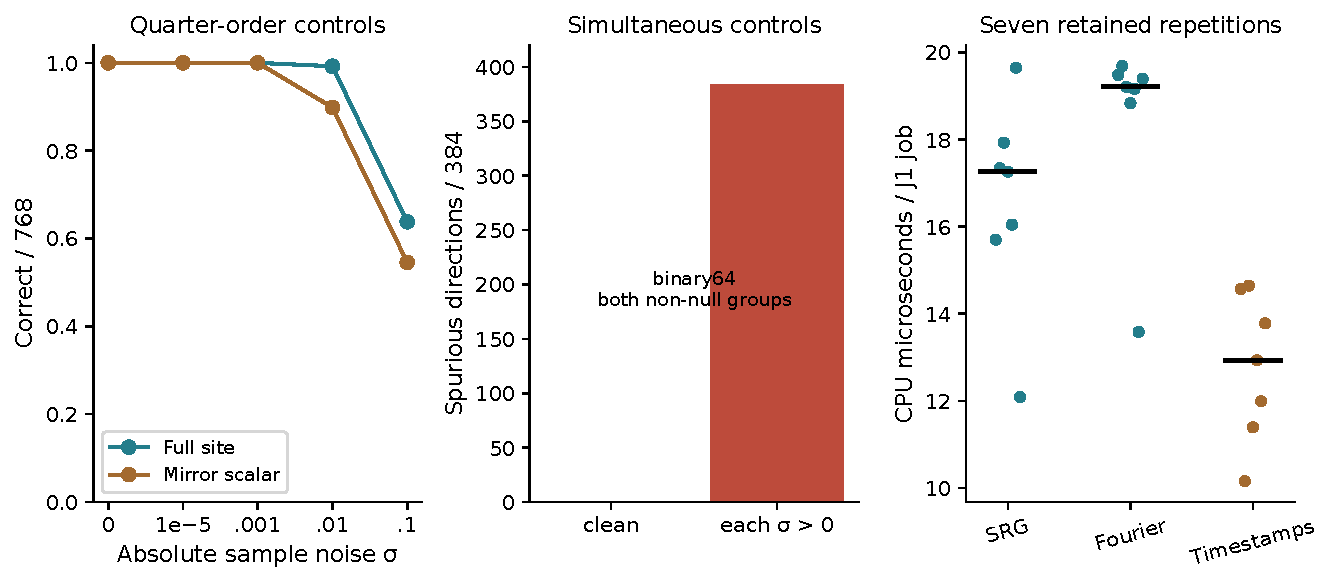
\includegraphics[width=\linewidth]{figures/fig03_measurements.pdf}
\caption{Retained corrected-run data: quarter-order noise accuracy, false simultaneous directions, and all seven J1 timing repetitions. Black timing marks are medians, not confidence intervals. Counts and time variability are distinct limits.}
\label{fig:measurements}
\end{figure}

\subsection{Two-run lineage and repeated-write evidence}
The pilot used Windows build 26200, an Intel64 Family 6 Model 183 Stepping 1 processor, 32 logical CPUs, Anaconda Python 3.11.15, NumPy 2.4.4 and QueryPerformanceCounter at reported 100 ns resolution. No CPU affinity, reserved host or hardware-energy counters were used. The first completed run took $51.44$ s with a reported 24-thread OpenBLAS configuration. Only a process configuration helper changed: it set thread variables before numerical imports, applied the existing pool limit and asserted the loaded thread count. The corrected run took $49.05$ s with one thread. The cause of the first launcher's missing variables was not established.

Both runs remain in the evidence. Three input corpora and eighteen saved data/summary files are byte-identical; timing, environment and elapsed metadata differ as expected. Only the corrected run supports the final timing claims. Per-directory no-rerun flags do not erase this two-run history. The original 178 checks, 26 result audits and later reviewer checks are inherited evidence, not newly executed manuscript tests.

At $N=128$, binary64 aligned alternating streams give zero coverage; aligned random orders give 54/96 correct with 89/96 covered. Random per-pair phases give 49/96 correct for alternating orders and 50/96 for random orders, with full coverage. Constant-label streams give 96/96 in either phase policy. These results agree with aggregation rather than universal recency.

The retained fixed-point subset is more striking: all 48 aligned random histories at length 128 are correct in directional coordinates at each width, while the Fourier path abstains on all 48. Every stream saturates; maximum coordinate-overflow counts are about 718--720 versus 477--479. The mean is below two instead of 128. The same histories are reused across widths, so these are not 144 independent successes. The next sections explain this distinct nonlinear effect and its failures.
